\documentclass[12pt]{article}
\usepackage{amsmath,mathtools}
\usepackage[usenames,dvipsnames]{xcolor}
%\usepackage[bitstream-charter]{mathdesign}
%\usepackage{mathptmx}

\usepackage{textcomp}
\usepackage{cmbright}
\usepackage[german]{babel}
\usepackage{microtype}
%\usepackage{microtype}
\usepackage[utf8]{inputenc}
\usepackage[T1]{fontenc}
\usepackage{helvet}
\renewcommand{\familydefault}{\sfdefault}

\usepackage{siunitx}
%\usepackage{tikz}
\usepackage{fancyhdr}
\usepackage{sectsty}
\usepackage{setspace}
\usepackage{booktabs} % To thicken table lines
\usepackage[version=4]{mhchem}
\usepackage{textcomp}
\usepackage{tabularx}
\usepackage[ddmmyyyy]{datetime}
\renewcommand{\dateseparator}{.}
\usepackage{geometry}
 \geometry{
 a4paper,
 left=20mm,
 top=30mm,
 right=30mm
 }


\pagestyle{fancy}

\cfoot{\thepage}

\lhead{Nevroz Arslan }
\rhead{\today}
\setlength{\headheight}{15pt}

\usepackage{overcite}
\renewcommand\citeform[1]{[#1]}

%\renewcommand*\printatom[1]{{\fontsize{10}{12}\selectfont\ensuremath{\mathsf{#1}}}}
\sectionfont{\fontsize{12}{15}\selectfont}

\makeatletter
    \setlength\@fptop{0\p@}
\makeatother


\newcommand\textbox[1]{%
  \parbox{.333\textwidth}{#1}%
}


\setlength{\headheight}{15pt}
\sisetup{detect-weight=true, detect-all}
\sisetup{text-celsius = $^\circ\mkern-1mu$C}


\renewcommand{\thesection}{\arabic{section}.}
\renewcommand{\thesubsection}{\thesection\arabic{subsection}}
\renewcommand{\headrulewidth}{0pt}

\begin{document}
%%%%%%%%%%%%%
\begin{onehalfspace}

\begingroup
\leftskip=0cm plus 0.5fil \rightskip=0cm plus -0.5fil
\parfillskip=0cm plus 1fil
 \textbf{\large Darstellung von 7-Methyl-3,3-diphenylazepan}\par
\endgroup

\begin{center}
 \textbf{Präparat Nr. 6 von 7}
\end{center}
\section{Reaktionstyp: \textnormal{Intramolekulare Hydroaminierung} }
\begin{figure}[ht]
\centering
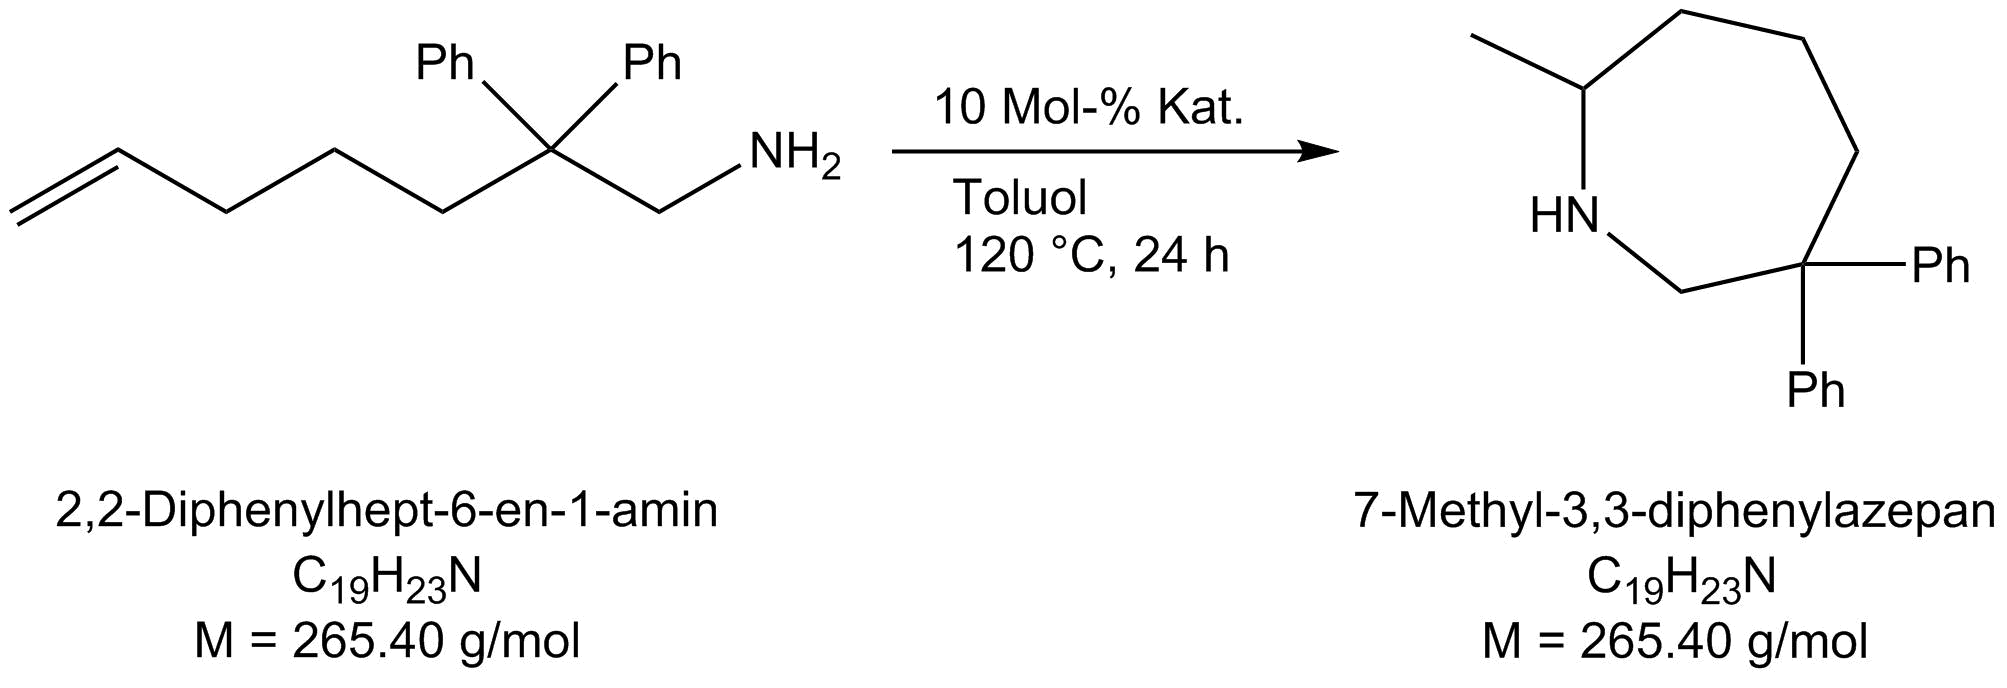
\includegraphics[scale=0.3]{reaktion.png}
\end{figure}

\section{Berechnung des Ansatzes: }
Es sollte 7-Methyl-3,3-diphenylazepan aus 2,2-Diphenylhept-6-en-1-amin (625 \si{\milli\gram}, 2.4\si{\milli\mol}) hergestellt werden. Die Umrechnung des Literaturansatzes ergab folgenden Ansatz:\cite{vor}\\\\
\noindent
\begin{tabularx}{\textwidth}{Xrrrr}
\toprule
\textbf{ Bezeichnung }&\textbf{M [\si{\gram\per\mol}]} & \textbf{ n [\si{\milli\mol}]} & \textbf{Menge [\si{\milli\gram}]}& \textbf{Equiv}\\
\midrule
 2,2-Diphenylhept-6-en-1-amin                    & 265.40   & 2.4  & 625  & 1.00 \\
 Tris(dimethylamido)(trityl(6-(tritylamino)pyridin-2-yl)amido)-titanium    & 772.86   & 0.1  & 77   & 0.04 \\
 Toluol &   &  & 2 \si{\milli\liter} & LM \\
\bottomrule
\end{tabularx}\\
%%%%%%%%%%%%%
% Durchführung
%%%%%%%%%%%%%
\section{Durchführung \cite{vor}}
In der Glove-Box wurden 2,2-Diphenylhept-6-en-1-amin (625 \si{\milli\gram}, 2.4 \si{\milli\mol}) und Toluol (1 \si{\milli\liter}) in einem 50 ml Schlenk-Rohr vorgelegt. Danach der Tris(dimethylamido)(trityl(6-(tritylamino)pyridin-2-yl)amido)-titanium zugegeben und im Rohr verbliebene Edukte werden mit Toluol (1 \si{\milli\liter}) nachgespült. Das Reaktionsgemisch wurde bei 120 \si{\celsius} 24~Stunden lang rühren gelassen und dann abgekühlt. Danach wurde das Gemisch mit \ce {CH_2Cl_2} (20~\si{\milli\liter}) hydrolysiert und am Rotationsverdampfer eingeengt. Das Rohprodukt 
wurde säulenchromatographisch (\ce{SiO_2} PE/EE = 30:1 $\rightarrow$ EE, \textit{R}\textsubscript{f}=0.15) gereinigt. Das Produkt (610 \si{\milli\gram}, 2.3 \si{\milli\mol}, 97 \%) wurde als farblose Flüssigkeit erhalten.
%%%%%%%%%%%%
% Ausbeute
%%%%%%%%%%%%%
\section{Ausbeute}
\begin{tabular}{ ll}
  625 \si{\milli\gram} (2.4 \si{\milli\mol})   & = 100 \%\\
  610 \si{\milli\gram} (2.3 \si{\milli\mol})   & = 97 \% (Lit.\cite{vor} (105 \si{\celsius}, 24 h): 75 \%) \\
 \end{tabular}
%%%%%%%%%%%%%
%Physikalische Daten des Produktes
%%%%%%%%%%%%%
%\section{Physikalische Daten des Produktes}
%\textit{2,2-Dimethyl-pent-4-enenitril}

\section{Spektrenauswertung}
\begin{figure}[!htbp]
   \centering
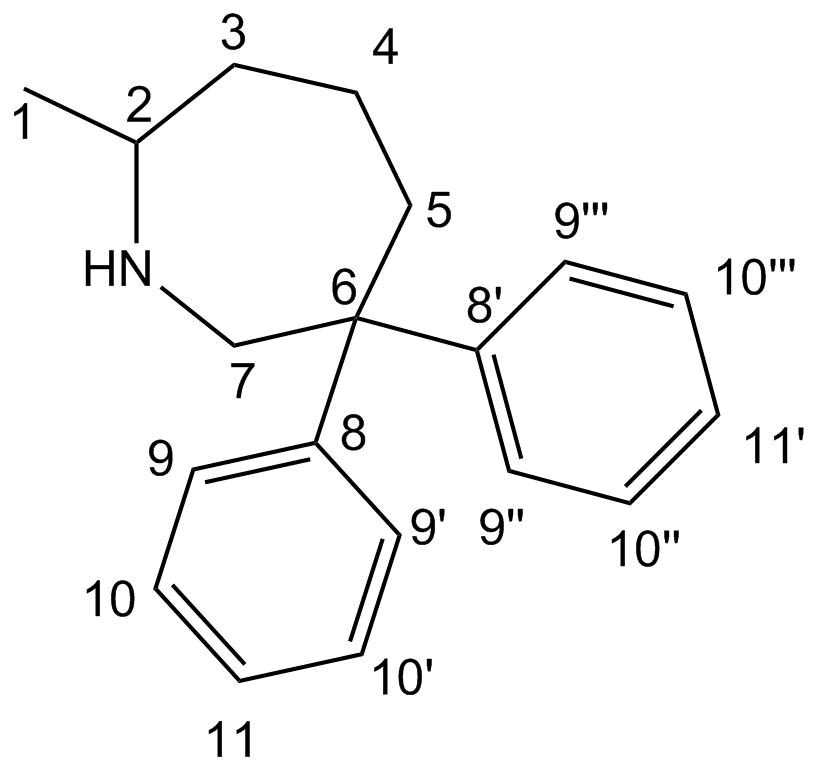
\includegraphics[scale=0.3]{auswert.png}
\end{figure}
\noindent
\textbf{\ce{^1_{}H-NMR}} (500 MHz, \ce{CDCl_3}): \sffamily \ce{$\delta$} =
1.01 (d, \ce{^3_{}\textit{J}} = 6.4 \si{\hertz}, 3 H, 1-H),
1.07 - 1.28 (m, 1 H, 3-H),
1.42 (br.S., 1 H, N-H),
1.57 - 1.67 (m, 1 H, 4-H),
1.69 - 1.87 (m, 2 H, 3-H, 4-H),
1.99 - 2.12 (m, 1 H, 5-H),
2.50 (dd, \ce{^3_{}\textit{J}} = 8.3 \si{\hertz}, \ce{^3_{}\textit{J}} = 14.8 \si{\hertz}, 1 H, 5-H),
2.67 - 2.82 (m, 1 H, 2-H),
3.01 (d, \ce{^3_{}\textit{J}} = 14.7 \si{\hertz}, 1 H, 7-H),
3.82 (d, \ce{^3_{}\textit{J}} = 14.7 \si{\hertz}, 1 H, 7-H),
7.03 - 7.23 (m, 6 H, 9-H, 10-H, 11-H) ppm. \\
\noindent
\textbf{\ce{^{13}_{}C-NMR}} (125 MHz, DEPT, \ce{CDCl_3}): \sffamily \ce{$\delta$} =
22.9 (\ce{CH_2}, C-4),
23.4 (\ce{CH_3}, C-1),
40.1 (2 x \ce{CH_2} , C-3, C-5),
52.3 (\ce{C}, C-6),
56.6 (\ce{CH}, C-2),
57.4 (\ce{CH_2}, C-7),
125.5 + 125.7 + 127.3 + 127.5 + 128.1 (10 x \ce{CH}, C-9, C-10, C-11)
148.2 + 150.1 (2 x \ce{C}, C-8) ppm. \\
\section{Mechanismus\cite{bio}}
Im Zuge der katalytischen Hydroaminierung erfolgt zunächst die Anlagerung des eingesetzten Amins \textbf{2} an den Titankomplex \textbf{1} unter Abspaltung eines Dimethylamino-Liganden. Durch weitere Abspaltung eines Dimethylamino-Liganden bildet sich eine katalytisch aktive Imido-Spezies \textbf{3}. An den Imido-Komplex \textbf{3} koordiniert dann die Alken-Gruppe des Aminoalkens. Es entsteht dabei eine Zwischenstufe, welche über eine [2+2] Cycloadditon ein Titanazacyclobutan \textbf{4} bildet. Im Anschluss wird der am Titan gebundene Kohlenstoff unter Öffnung des Cyclobutan-Rings protoniert. Es entsteht dabei eine Amido-Spezies \textbf{5}. In dem nächsten Schritt des Zyklus wird das gewünschte Produkt 7-Methyl-3,3-diphenylazepan (\textbf{6}) unter Koordinaton des Ausgangstoffes \textbf{2} an die Amido-Spezies \textbf{6} abgespalten und aus dem Katalysezyklus entfernt. Es wird dabei die katalytisch aktive Imido-Spezies \textbf{3} ausgebildet. Damit wird der katalytische Zyklus erneut gestartet.\\
\newpage
\begin{figure}[!htbp]
\centering
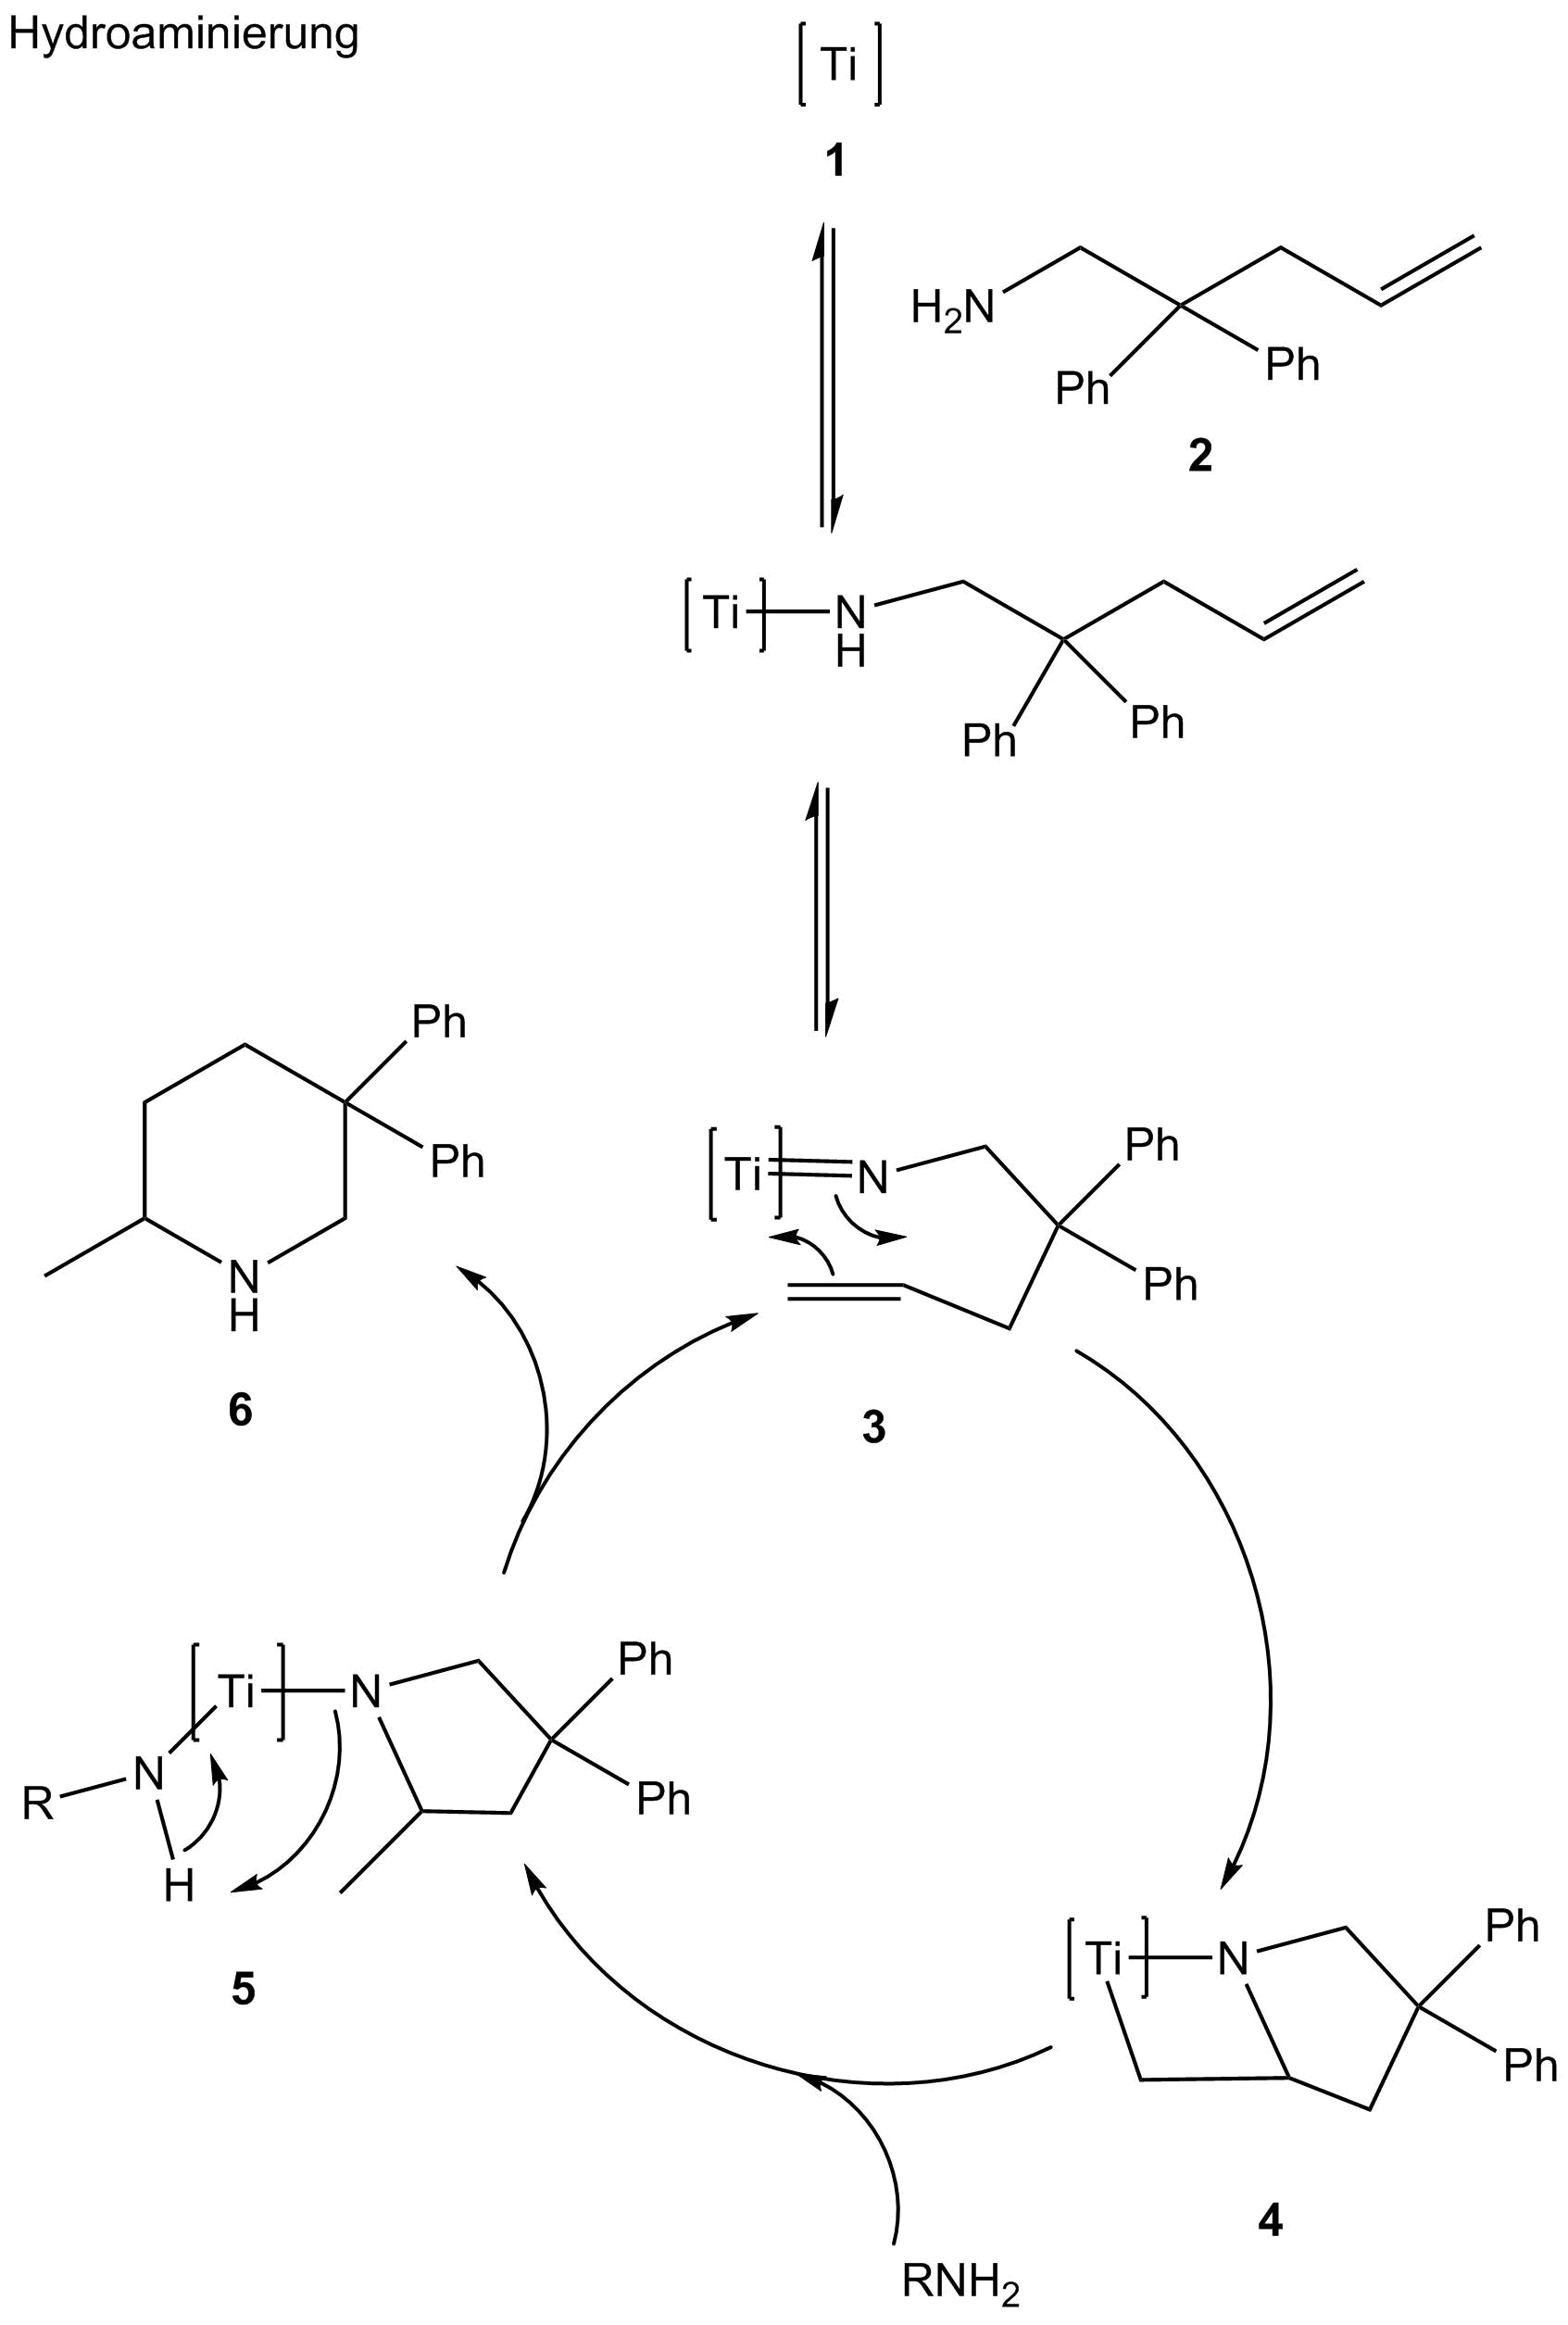
\includegraphics[width=0.9\textwidth]{kat.png}
\end{figure}

\section{Abfallentsorgung}
Das im Rotationsverdampfer abgetrennte Lösungsmittel wurde im Behälter für halogenhaltige Kohlenwasserstoffe entsorgt.
Das nach der Säulenchromatographie abgetrennte Lösungsmittel wurde im Behälter für halogenfreie Kohlenwasserstoffe entsorgt.
\section{Literatur}

\renewcommand{\section}[2]{}%
\def\bibindent{0em}
\begin{thebibliography}{99\kern\bibindent}
\makeatletter
\let\old@biblabel\@biblabel
\def\@biblabel#1{\old@biblabel{#1}\kern\bibindent}
\let\old@bibitem\bibitem
\def\bibitem#1{\old@bibitem{#1}\leavevmode\kern-\bibindent}
\makeatother
\bibitem{vor}
L. H. Lühning, C. Brahms, J. P. Nimoth, M. Schmidtmann, S. Doye, \textit{Z. anorg. allg. Chem.} \textbf{2015}, \textit{641}, 2071–2082.
\bibitem{bio}
C. Müller, R. Koch, S. Doye, \textit{Chem. Eur. J.} \textbf{2008}, \textit{14}, 10430–10436.
\end{thebibliography}
\end{onehalfspace}
\end{document}


%http://onlinelibrary.wiley.com/doi/10.1002/chem.200801445/full
%http://onlinelibrary.wiley.com/doi/10.1002/1521-3757%2820010618%29113:12%3C2361::AID-ANGE2361%3E3.0.CO;2-J/full